%# -*- coding: utf-8-unix -*-
%%==================================================
%% software requirement specification
%%==================================================
%\bibliographystyle{sjtu2}%[此处用于每章都生产参考文献]


%\usetikzlibrary{trees}
\usetikzlibrary{arrows,shapes,positioning,shadows,trees}
\tikzstyle{every node}=[draw=black,thick,anchor=west]
\tikzstyle{selected}=[draw=red,fill=red!30]
\tikzstyle{optional}=[dashed,fill=gray!50]

\chapter{相似轨迹查询系统需求分析}
\label{chap:system requirement specification}

\section{本章序言}
\label{sec:requirement introduction}
本文中,相似轨迹查询系统需求分析需要明确:在该查询系统中,针对不同的用户类型提供的轨迹查询点集或者一条历史轨迹输入,在满足系统交互原则的基础上,准确高效通过可视化的方式输出系统所处理出的相似轨迹结果。

\section{需求分析背景概述}
\label{sec:requirement background}
目前相似轨迹查询这一领域的研究成果在学术方面有着丰富和较为系统的成果,不过目前这些学术成果移植到系统应用中的样例较为稀缺。在国内开发的地图应用或者提供以地图搜索为主体的公司在相似轨迹查询这一领域所投入的精力并不多,导致基于相似轨迹查询的系统软件发展投入在实际应用中的比例相对较少。

\subsection{系统应用定位分析}
\label{subsec:system orientation}
相似轨迹查询系统软件设计的初始主要目标为外出旅游对景点进行路径规划、外出前查询起始地点路径和进行日常拼车需求的轨迹数据使用用户。由于社会人员拥有私有交通工具的比例上升以及配置GPS轨迹设备的流行性,越来越多的用户需要借助可视化的轨迹数据管理方法来查询和管理自己的轨迹数据,其中相似轨迹查询便是其中需求之一。相似轨迹查询问题可以在上述的三种初始应用中,借助系统内部的地图可视化接口,满足用户需求。

\subsection{系统应用范围}
\label{subsec:scope}
相似轨迹查询系统是一个基于\emph{GPS}轨迹数据的服务器端应用系统。根据轨迹用户提供的输入轨迹或一组基于GPS数据的轨迹点集,系统帮助用户在地理语义上查询出与输入最相似的k条结果轨迹。系统可以免费从Github上下载并运行在可以运行Python程序的平台上。

本系统在应用中,需要连接互联网以调用基于Javascript的地图服务接口,实现地图显示和轨迹显示等等基础功能。所有系统所需要的轨迹数据以文件系统存储于服务器端。在系统运行过程中,用户可以通过浏览器登录页面进行系统访问,结合用户自身查询需求系统得出不同的查询结果。本系统也支持展示出所有地图上具体位置信息和查询具体地理位置的功能。

\subsection{系统可行性分析}
\label{subsec:system feasibility}
本文通过搭建Web框架实现相似轨迹查询系统,从如图\ref{fig:feasibility}几个方面阐述搭建相似轨迹查询系统在用户人群中使用的可行性:
\begin{itemize}
	\item 网络应用基础设施完善:现在在中国,互联网的发展使得人们可以通过PC终端和移动端访问各类网站。网络应用在企业公司和家庭用户中都有着广泛的普及,这为用户方便使用相似轨迹查询系统提供可能性。
	\item 地图数据处理数据优秀:在国内外诸如谷歌地图、百度地图和高德地图等等公司提供的基于各种开发平台的地图应用程序接口使得系统开发人员能够跨平台的开发出各种有关地图数据的应用。且各种接口功能丰富,性能优秀,可视化程度良好。
	\item 轨迹数据规模庞大:轨迹数据生成和处理技术的成熟发展使得系统所存储的轨迹数据规模在一定的用户使用规模上是具备大数据规模的,使得系统通过相似轨迹处理得到结果的准确性和实用性进一步得到保证。
	\item 网络应用技术普及:网络技术、Web技术、各种网络数据库技术的发展为本文开发基于Web框架的系统软件提供可能性,这些主流技术的系统发展是本文开发与设计系统的主要支持,为本文系统的实现提供保障。
\end{itemize}

\vspace{3mm}

\begin{figure}[!htp]
    \centering
    \resizebox{!}{!}{
\begin{tikzpicture}[%
  grow via three points={one child at (0.5,-0.7) and
  two children at (0.5,-0.7) and (0.5,-1.4)},
  edge from parent path={(\tikzparentnode.south) |- (\tikzchildnode.west)}]
  \node {系统可行性依赖}
    child { node {网络应用基础设施完善}}		
    child { node {地图数据处理数据优秀}}
    child { node {轨迹数据规模庞大}}
    child { node {网络应用技术普及}};
\end{tikzpicture}}
    \bicaption[fig:feasibility]{相似轨迹查询系统可行性}{相似轨迹查询系统可行性}{Fig}{Feasibility of searching similar trajectories system}
\end{figure}

\section{系统需求综述}
\label{sec:overall description}
在开展相似轨迹查询系统设计之前,我们首先对要设计的系统所涉及的实际需求进行描述。在定义好该系统所需要解决的应用问题和需要满足的用户需求之后,在因地制宜设计系统框架。

\subsection{系统需求背景}
\label{subsec:general requirements}
随着GPS技术不断发展和私家车数量的激增,生活中每天都会产生海量数据规模的轨迹数据。用户想要根据特定需求查询轨迹(例如本文所要解决的查询相似轨迹),通过传统的软件系统难以高效查询出所期望的结果。我们通过基于目前主流的算法实现,设计出快速、准确的相似轨迹查询系统,借助网页地图接口将查询结果清晰了然展示在用户界面上。系统在实现相似轨迹查询的基础上,可以为用户提供轨迹路径规划和轨迹推荐等基于相似轨迹查询的应用服务。

\subsection{系统需求说明目的}
\label{subsec:propose}
在完成对相关工作的研究和系统市场的前景分析后,本文提出相似轨迹查询系统设计需求说明。相似轨迹查询查询系统设计需求说明的目的在于对于本系统进行具体描述,明确索要开发的系统应该具备的功能与界面,为系统分析及移植开发提供清晰的基础需求描述,并以此为基础进一步满足后续设计与开发。本文所设计开发的相似轨迹查询系统目标是为用户提供高效、准确的查询服务平台。系统针对目前轨迹信息管理的实际情景,较为全面地满足用户的查询需求,初步实现系统所制定的设计初衷。需求说明从字面上作为软件系统发展的指导和完备部分,解释说明了系统中的限制条件、应用交互接口以及具体功能。

\subsection{系统设计分析}
\label{subsec:system build requirement}
将相似轨迹查询系统以Web框架搭建,其最大的好处是给予用户在查询上最大程度的便利。这种便捷主要体现在用户只要连接上互联网,就可以直接通过浏览器访问系统,在线进行相似轨迹的查询。这种网络操作不需要用户在下载系统到终端或者移动端便可以进行实时的相似轨迹查询功能。所以在设计相似轨迹查询这一系统时,主要功能实现均为用户查询而服务,即最重要的一点是完成用户功能部分。


%%%%%%%%%%%%%%%%%%%%


\section{功能需求}
\label{sec:function requirements}

\subsection{用户功能需求}
\label{subsec:user class functional requirements}
\begin{enumerate}
   \item 一般查询用户:
   \begin{itemize}
   		\item 基于轨迹点集的相似轨迹查询功能:一般查询用户在地图界面上点击地理位置或根据查询输入窗口输入查询地点,同时可以增加或删除查询点。查询轨迹点集会以小图标的形式显示上地图上。结合查询日期条件,搜索出相似轨迹。
   \end{itemize}
   \item 登录用户:
   \begin{itemize}
		\item 登录功能:登录用户ID和密码登录到用户界面,显示用户的历史轨迹。
		\item 显示历史轨迹数据功能:登录用户可以选择一条历史轨迹数据,展示与地图上
		\item 基于历史轨迹的相似轨迹查询功能:在选择一条历史轨迹时候,登录用户在设定好查询时间参数后可以进行相似轨迹查询功能。
		\item 基于轨迹点集的相似轨迹查询功能:一般查询用户在地图界面上点击地理位置或根据查询输入窗口输入查询地点,同时可以增加或删除查询点。查询轨迹点集会以小图标的形式显示上地图上。结合查询日期条件,搜索出相似轨迹。
   \end{itemize}
\end{enumerate}

\vspace{3mm}


\begin{figure}[!htp]
    \centering
    \resizebox{!}{!}{
%\begin{tikzpicture}[node distance=2cm]
%	\node (user) [startstop] {用户};
%	\node (n1) [process, left of=user, xshift=-2cm]{历史轨迹查询};
%	\node (n2) [process, above of=user]{注册和登录};
%	\node (n3) [process, right of=user, xshift=2cm]{相似轨迹查询};
%	\node (n4) [process, below of=user]{地理位置查找};
%	
%	\draw [arrow] (user.west) -- (n1.east);
%	\draw [arrow] (user.east) -- (n3.west);
%	\draw [arrow] (user.north) -- (n2.south);
%	\draw [arrow] (user.south) -- (n4.north);
%\end{tikzpicture}

\begin{tikzpicture}[%
  grow via three points={one child at (0.5,-0.7) and
  two children at (0.5,-0.7) and (0.5,-1.4)},
  edge from parent path={(\tikzparentnode.south) |- (\tikzchildnode.west)}]
  \node {用户功能需求}
    child { node {注册和登录}}		
    child { node {相似轨迹查询}}
    child { node {历史轨迹查询}}
    child { node {地理位置查找}};
\end{tikzpicture}

}
    \bicaption[fig:user-func]{相似轨迹查询系统用户功能需求}{相似轨迹查询系统用户功能需求}{Fig}{User function requirement in the system}
\end{figure}

\subsection{用户界面需求}
\label{subsec:external interface Requirements}
\begin{itemize}
	\item 用户登录界面:实现用户账户与密码登录。
	\item 功能选择界面:进入相似轨迹查询系统后选择用户所需要的功能。
	\item 地图显示界面:在一般用户和登录用户模式中都可以显示城市地图信息,通过高德地图\cite{AutoNavi}接口实现附属界面功能。
	\item 地理位置点输入界面:在输入界面中输入地址位置名称,显示对应的地理经纬度坐标并在地图上显示具体位置。
	\item 查询条件设定界面:相似轨迹查询窗口,结合用户自定义条件作为相似轨迹查询的附属输入参数。
	\item 历史轨迹显示界面:显示登录用户的历史轨迹数据条目。
\end{itemize}

%\begin{figure}[!htp]
%    \centering
%    \resizebox{!}{!}{\begin{tikzpicture}[%
  grow via three points={one child at (0.5,-0.7) and
  two children at (0.5,-0.7) and (0.5,-1.4)},
  edge from parent path={(\tikzparentnode.south) |- (\tikzchildnode.west)}]
  \node {用户界面需求}
    child { node {用户登录界面}}		
    child { node {功能选择界面}}
    child { node {地图显示界面}}
    child { node {查询条件设定界面}}
    child { node {历史轨迹显示界面}}
    child { node {地理位置点输入界面}};
\end{tikzpicture}}
%    \bicaption[fig:interface-func]{相似轨迹查询用户界面需求}{相似轨迹查询用户界面需求}{Fig}{User interface requirement in the system}
%\end{figure}

\vspace{3mm}

\begin{figure}[!htp]
    \centering
    \resizebox{!}{!}{\begin{tikzpicture}[%
  grow via three points={one child at (0.5,-0.7) and
  two children at (0.5,-0.7) and (0.5,-1.4)},
  edge from parent path={(\tikzparentnode.south) |- (\tikzchildnode.west)}]
  \node {用户界面需求}
    child { node {用户登录界面}}		
    child { node {功能选择界面}}
    child { node {地图显示界面}}
    child { node {查询条件设定界面}}
    child { node {历史轨迹显示界面}}
    child { node {地理位置点输入界面}};
\end{tikzpicture}}
    \bicaption[fig:interface-func]{相似轨迹查询用户界面需求}{相似轨迹查询用户界面需求}{Fig}{User interface requirement in the system}
\end{figure}

\section{性能需求}
\label{sec:performance requirements}

\subsection{系统查询准确率}
\label{subsec:performance accuracy}
相似轨迹查询应保证查询结果与输入轨迹数据相似度较高。在地理语义上,相似轨迹查询结果应该尽可能地靠近查询输入点集或是输入轨迹。以图\ref{fig:accuracy}为例,其中$T1$,$T2$和$T3$是历史轨迹,轨迹查询点集为圆圈表示,从图中我们可以看出$T1$相对于$T2$和$T3$,是更相似于输入的历史轨迹,因此在系统查询中,若以上述查询点集作为输入,首先应输出$T1$以保证查询准备率。

\begin{figure}[!htp]
  \centering
  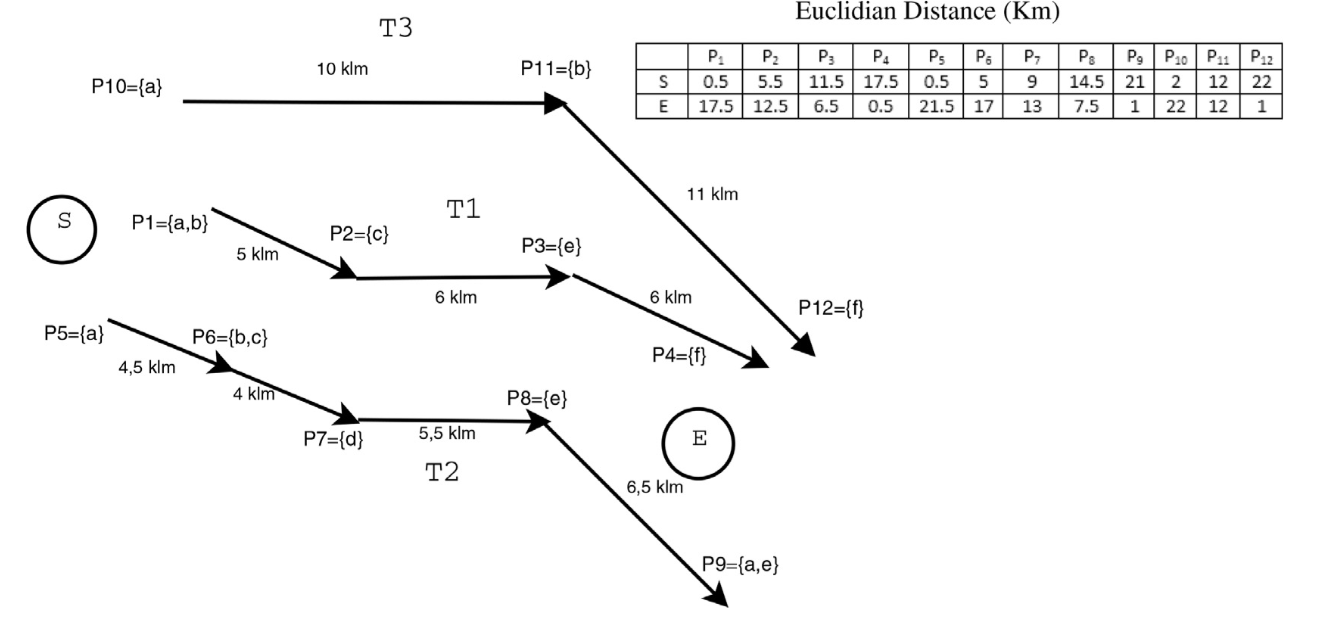
\includegraphics[width=0.75\textwidth]{requirement/query-accuracy.png}
  \bicaption[fig:accuracy]{系统查询结果准确性}{系统查询结果准确性}{Fig}{Accuracy of searching}
\end{figure}

\subsection{系统查询时间特性}
\label{subsec:performance time}
在相似轨迹查询系统中,单机查询点集操作普遍在一秒内完成;若输入点过多或者以一条轨迹作为查询输入,所需的查询时间会到两秒。在交互型系统中,这样这时间操作在可接受范围之内。

\subsection{系统适应性}
\label{subsec:performance flexibility}
相似轨迹查询系统可以根据用户特定的查询需求满足有序或无序、有关轨迹日期、查询数目限制等类型。在满足运行条件的情况可正常运行于各种场景。

\section{本章小结}
\label{sec:requirement conclusion}
系统软件需求分时是在对系统如何开发的概要描述。本章节主要针对相似轨迹查询系统在目前研究环境中,要解决的主要问题进行相似的需求分析,明确系统的问题要求,了解输入与输出,并从用户的角度描述了系统应该具备哪些实际的功能,达到什么的性能标准。与此同时,本章节内容也分析了相似轨迹查询系统在功能性与非功能性中的大致组成框架,为从事相关领域的软件工程师确定用户的基本使用需求。在明确这些需求之后,本文才开始对相似轨迹查询系统进行针对性的设计与构思,为下一章节相似轨迹查询系统的设计与实现提供基础。
